\documentclass{article}
\usepackage[utf8]{inputenc}
\usepackage[spanish]{babel}
\usepackage{listings}
\usepackage{graphicx}
\usepackage{cite}

\begin{document}

\begin{titlepage}
    \begin{center}
        \vspace*{1cm}
            
        \Huge
        \textbf{Proyecto Final}
            
        \vspace{0.5cm}
        \LARGE
        Los primeros pasos
            
        \vspace{1.5cm}
            
        \textbf{Miguel Ángel Alvarez Guzmán}
            
        \vfill
            
        \vspace{0.8cm}
            
        \Large
        Departamento de Ingeniería Electrónica y Telecomunicaciones\\
        Universidad de Antioquia\\
        Medellín\\
        Marzo de 2021
            
    \end{center}
\end{titlepage}

\tableofcontents
\newpage
\section{Introducción.}\label{intro}
El propósito de este documento es dar a conocer la forma de implementación de las clases que se van a dar en el juego para presentarlo en informática ii en el entorno C++ junto con su cronograma respectivo.
\section{Clases.} \label{contenido}
\subsection{Clases de interfaz.}
Se incluirán todas las clases correspondientes con el motor gráfico de QTcreator para poder trabajar la interfaz de la forma mas acorde a lo planteado por los docentes.
\subsection{Clases de cámara.}
Se tomara la cámara como una clase en especifico para poder manipularla al antojo y así lograr un comportamiento óptimo entre la iluminación y el movimiento de los personajes.
\subsection{Clases de personajes.}
Sera la clase mas principal por decirlo de algún modo en la cual se dará los factores de movimiento a los personajes y sus físicas.
\subsection{Clases extra.}
Se implementaran mas clases dentro del desarrollo pero estas no se tomaran en cuenta ya que no son tan representativas.
\vspace{5.2cm}
\section{Cronograma.}

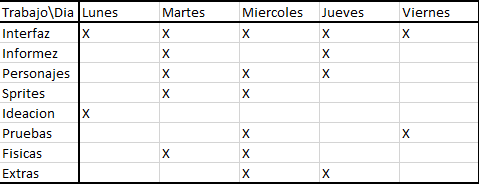
\includegraphics[width=\textwidth]{Cronograma.png}

\end{document}
